%!TEX root=../protocol.tex	% Optional
\section{Architektur}

Die Anwendung ``Gschäftlhaberer'' soll wie folgt aufgebaut werden:

\vspace{1em}

\begin{figure}
    \centering
	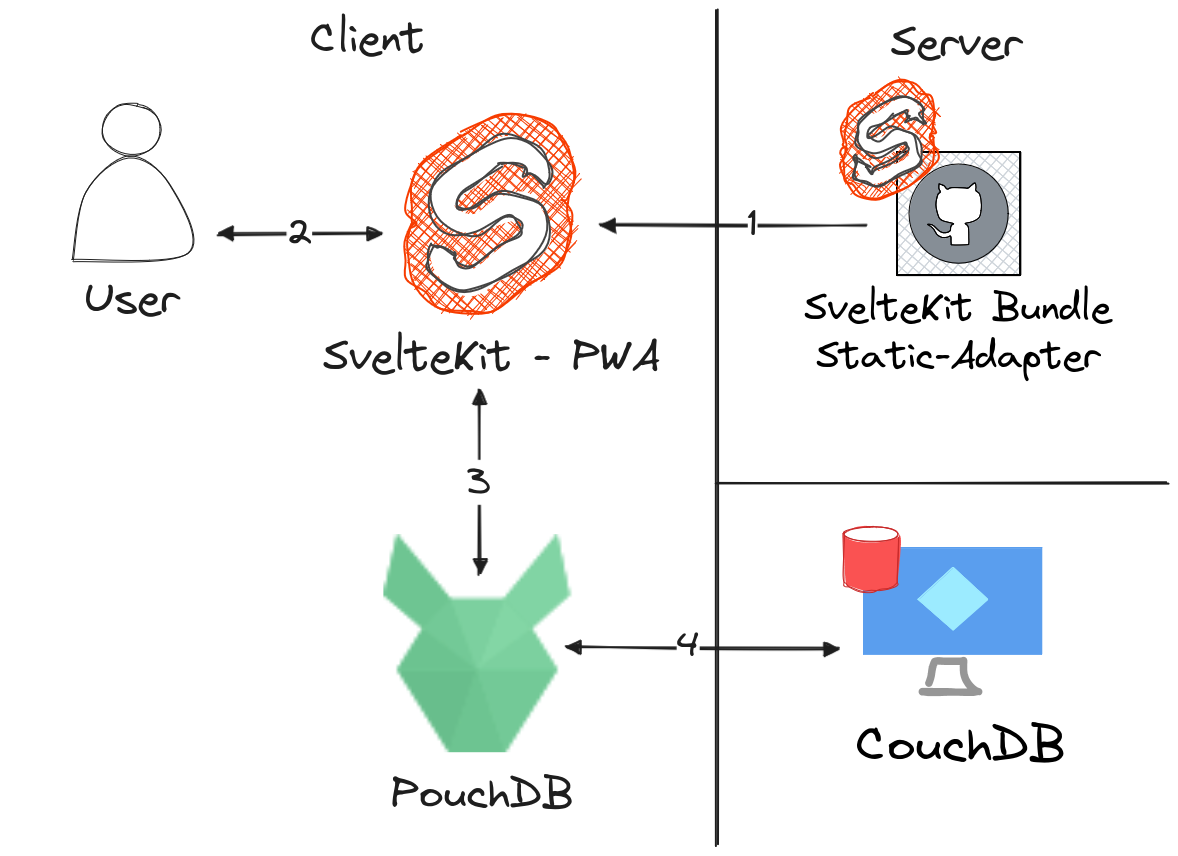
\includegraphics[width=0.8\textwidth]{images/architecture.png}
    \caption{Ein Übersicht über die Komponenten und Dienste in Gschäftlhaberer}\cite{shopping-list:architecture}
\end{figure}

Zuerst wird die Anwendung in Form eines SvelteKit Static-Adapter Bundles, bestehend aus HTML, CSS und Javascript Dateien, von einem statischen Webserver (GitHub Pages) heruntergeladen (1). Diese Datei registiert sich angschlie{\ss}end im Browser als Webworker und richtet einen Cache für die Anwendungsdateien ein, um Offline-Verfügbarkeit zu ermöglichen. Optional kann sie hier auch als PWA (Progressive Web App installiert werden). Der Nutzer interagiert mit diser im Browser gezeigten Anwendung (2), welche als Daten-Basis eine im Browser laufende PouchDB-Instanz verwendet (3). Um die Einkaufsliste anschließend teilen zu können, kann sie auf eine CouchDB Instanz synchronisiert werden (4).

\subsection{Gewählte Technologien}

\begin{description}
    \item[SvelteKit\cite{sveltekit}] verzichtet im Gegensatz zu Ansätzen wie Vue und React auf einen virtuellen DOM und compiled stattdessen den Code in Vanilla-JS Code, der direkt mit dem Browser DOM integriert.\cite{svelte} Außerdem bietet SvelteKit eine integrierte Möglichkeit einen Service-Worker zu installieren.\cite{sveltekit:serviceworker}
    \item[CouchDB\cite{couchdb}] ist eine Dokument basierte NoSQL Datenbank, die ein RESTful API bereitstellt. Sie ist für die Synchronisation von Daten zwischen verschiedenen Geräten ausgelegt.\cite{couchdb}\cite{couchdb:overview}
    \item[PouchDB\cite{pouchdb}] ist eine Javascript Datenbank, welche als Speicher Browser APIs verwendet und damit in WebApps verwendet werden kann. Zusätzlich bietet sie eine Möglichkeit mit CouchDB kompatiblen Datenbanken zu synchronisieren.\cite{pouchdb:about}
\end{description}
